\documentclass{article}
\usepackage{tikz}
\usetikzlibrary{hobby,shapes,arrows,fit,calc,positioning} 
\begin{document}
	\begin{center}
	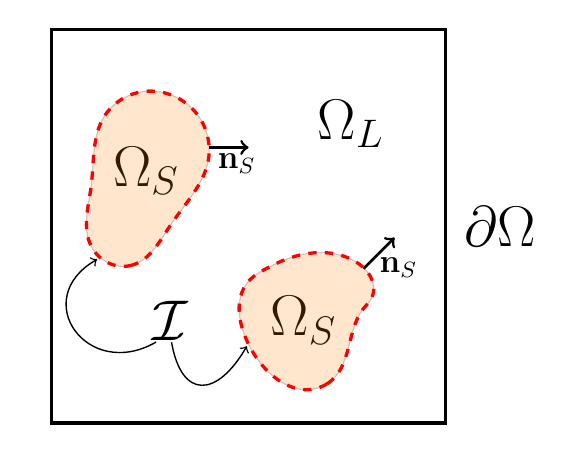
\begin{tikzpicture}
	
	
	\draw[arrows=->,line width=1pt](2,3.5)--(2.5,3.5);
	\node[draw=none,fill=none, xshift = 2.35cm, yshift= 3.3cm] {\large$\textbf{n}_S$}; 
	\node[draw=none,fill=none, xshift = 1.2cm, yshift= 3.2cm] {\huge$\Omega_S$}; 
	\node[draw=none,fill=none, xshift = 3.2cm, yshift= 1.3cm] {\huge$\Omega_S$}; 
	\node[draw=none,fill=none, xshift = 3.8cm, yshift= 3.8cm] {\huge$\Omega_L$}; 
	\node[draw=none,fill=none, xshift = 1.5cm, yshift= 1.3cm] {\huge$\mathcal{I}$}; 
	\node[draw=none,fill=none, xshift = 5.7cm, yshift= 2.5cm] {\huge$\partial\Omega$}; 
	\draw[black, very thick] (0,0)rectangle (5,5);
	
	\node (a) at(1.45, 1.1)  {};
	\node (b) at  (0.7, 2.15){};
	\draw[->,line width =0.5pt] (a)  to [out=-150,in=-150, looseness=2] (b);

	\node (c) at(1.5, 1.15)  {};
	\node (d) at  (2.55, 1.1){};
	\draw[->,line width =0.5pt] (c)  to [out=-80,in=600, looseness=2] (d);
	
	\begin{scope}[xshift = 1cm, yshift = 2cm,black]
	\path[draw,use Hobby shortcut,closed=true, fill = orange, opacity = 0.2]
	(0,0) .. (.5,.5) .. (1,1.5) .. (-.25,2) .. (-.5,1) .. (-.5,.25);
	\end{scope}
	\begin{scope}[xshift = 1cm, yshift = 2cm,red, very thick]
	\path[draw,,use Hobby shortcut,closed=true,dashed]
	(0,0) .. (.5,.5) .. (1,1.5) .. (-.25,2) .. (-.5,1) .. (-.5,.25);
	\end{scope}
	
	\draw[arrows=->,line width=1pt](3.96,1.96)--(4.354,2.354);
		\node[draw=none,fill=none, xshift = 4.4025cm, yshift= 1.975cm] {\large$\textbf{n}_S$}; 
	\begin{scope}[xshift = 3.5cm, yshift = .5cm,black]	
	\path[draw,use Hobby shortcut,closed=true,fill = orange, opacity = 0.2]
	(0,0) .. (.5,1) .. (.5,1) .. (-0.7,1.5) .. (-1,1.3) .. (-1,.5);
	\end{scope}
	\begin{scope}[xshift = 3.5cm, yshift = .5cm,red, very thick]	
	\path[draw,use Hobby shortcut,closed=true,dashed]
	(0,0) .. (.5,1) .. (.5,1) .. (-0.7,1.5) .. (-1,1.3) .. (-1,.5);
	\end{scope}
	\end{tikzpicture}
	\end{center}

\section{A-posteriori 2}
\subsection{Upper bound}
Consider a bilinear form $A$ and a linear form $B$,
\begin{eqnarray}
A&:&\left[\textbf{H}^1_0\right]^d\times\left[\textbf{H}^1_0\right]^d \rightarrow\mathbb{R}\text{ and}\\
B&:&\left[\textbf{H}^1_0\right]^d\times \left[\textbf{L}^2_0\right]\,\,\rightarrow\mathbb{R},
\end{eqnarray}
such that
\begin{eqnarray}
A\left(\textbf{u},\textbf{v}\right)&\coloneqq& \int_{\Omega}\nabla\textbf{u}:\nabla \textbf{v}\text{ and}\\
B\left(\textbf{v},q\right)&\coloneqq&-\int_{\Omega}q\,\text{div}\left(\textbf{v}\right).
\end{eqnarray}
The weak form of the Stokes equation is to find $\left(\textbf{u},p\right)\in \left[\textbf{H}^1_0\right]^d  \times \textbf{L}^2_0$ such that
\begin{equation}\label{weak_stokes}
\begin{rcases}
A\left(\textbf{u},\textbf{v}\right)+B\left(\textbf{v},p\right)&=F\left(\textbf{v}\right)\\
B\left(\textbf{u},q\right)&=0
\end{rcases}
\quad\forall \left(\textbf{v},q\right)\in \left[\textbf{H}^1_0\right]^d  \times \textbf{L}^2_0.
\end{equation}
The finite element approximation of this problem is to find $\left(\textbf{u}_h,p_h\right)\in \left[\mathbb{V}_1\right]^d  \times \mathbb{V}_2\eqqcolon\mathbb{W}$ such that
\begin{equation}\label{weak_stokes_approx}
\begin{rcases}
A\left(\textbf{u}_h,\textbf{v}_h\right)+B\left(\textbf{v}_h,p_h\right)&=F\left(\textbf{v}_h\right)\\
B\left(\textbf{u}_h,q_h\right)&=0
\end{rcases}
\quad\forall \left(\textbf{v}_h,q_h\right)\in \mathbb{W}.
\end{equation}
We now want to control the error for the velocity, $\textbf{e}_u$ and for the pressure, $e_p$.   At the moment we will just obtain an upper bound.  Let us begin by defining both the pressure and the velocity error:
\begin{eqnarray}\label{error_velocity}
\textbf{e}_u&=&\textbf{u}-\textbf{u}_h,\\\label{error_pressure}
e_p &=& p-p_h
\end{eqnarray}
In order to control this error we first choose $\textbf{v}=\textbf{v}_h\in\mathbb{V}_1$, $q=q_h\in\mathbb{V}_2$ in (\ref{weak_stokes}) and then we subtract (\ref{weak_stokes_approx}) from (\ref{weak_stokes}) to obtain
\begin{equation}\label{weak_stokes_approx_galerkin}
\begin{rcases}
A\left(\textbf{u}-\textbf{u}_h,\textbf{v}_h\right)+B\left(\textbf{v}_h,p-p_h\right)&=\textbf{0}\\
B\left(\textbf{u}-\textbf{u}_h,q_h\right)&=0
\end{rcases}\quad\forall \left(\textbf{v}_h,q_h\right)\in \mathbb{W}.
\end{equation}
This is just a way of saying that the error obeys Galerkin orthogonality.  We now want to change (\ref{weak_stokes_approx_galerkin}) to a form which is convenient in helping us establish a bound for the error.  We do this by manipulating the bilinear form $A$ and the linear form $B$:
\begin{equation}\small \label{weak_stokes_approx_error}
\begin{rcases}
A\left(\textbf{u}-\textbf{u}_h,\textbf{v}\right)+B\left(\textbf{v},p-p_h\right)&=A\left(\textbf{u}-\textbf{u}_h,\textbf{v}-\textbf{v}_h\right)+B\left(\textbf{v}-\textbf{v}_h,p-p_h\right)\\
B\left(\textbf{u}-\textbf{u}_h,q\right)&=B\left(\textbf{u}-\textbf{u}_h,q-q_h\right).
\end{rcases}\quad\forall \left(\textbf{v}_h,q_h\right)\in \mathbb{W}.
\end{equation}
In order to proceed we choose $\textbf{v}=\textbf{u}-\textbf{u}_h$ and $q=p-p_h$ in (\ref{weak_stokes_approx_error}).  This gives:
\begin{equation} \label{weak_stokes_error_bilinforms}
\begin{aligned}
\left|\textbf{u}-\textbf{u}_h\right|^2_1 &=A\left(\textbf{u}-\textbf{u}_h,\textbf{u}-\textbf{u}_h\right)-A\left(\textbf{u}-\textbf{u}_h,\textbf{v}_h\right)\\
&+B\left(\textbf{u}-\textbf{u}_h,p-p_h\right)-B\left(\textbf{v}_h,p-p_h\right)\\
&+B\left(\textbf{u}-\textbf{u}_h,p-p_h\right)-B\left(\textbf{u}-\textbf{u}_h,q_h\right)
\end{aligned}
\end{equation}
Now we make use of the error definitions (\ref{error_velocity}) and (\ref{error_pressure}) in (\ref{weak_stokes_error_bilinforms}) for convenience in the analysis that will follow:
\begin{equation} \label{weak_stokes_error_bilinforms_euep}
\begin{aligned}
\left|\textbf{e}_u\right|^2_1 &=A\left(\textbf{e}_u,\textbf{e}_u\right)-A\left(\textbf{e}_u,\textbf{v}_h\right)\\
&+B\left(\textbf{e}_u,e_p\right)-B\left(\textbf{v}_h,e_p\right)\\
&+B\left(\textbf{e}_u,e_p\right)-B\left(\textbf{e}_u,q_h\right).
\end{aligned}
\end{equation}
Let $\mathcal{I}_{\mathbb{V}_1}\textbf{e}_u$ and $\mathcal{I}_{\mathbb{V}_2}e_p$ be the approximations of $\textbf{e}_u$ and $e_p$  respectively in their associated finite element subspace.  Now let $\textbf{v}_h= \mathcal{I}_{\mathbb{V}_1}\textbf{e}_u$  and $q_h=\mathcal{I}_{\mathbb{V}_2}e_p$ in (\ref{weak_stokes_error_bilinforms_euep}) (and dropping the subspace subscripts from $\mathcal{I}_{\mathbb{V}_{\left(\cdot\right)}}$) to get 
\begin{equation} \label{weak_stokes_error_bilinforms_euIeu}
\begin{aligned}
\left|\textbf{e}_u\right|^2_1 &=A\left(\textbf{e}_u,\textbf{e}_u-\mathcal{I}\textbf{e}_u\right)\\
&+B\left(\textbf{e}_u-\mathcal{I}\textbf{e}_u,e_p\right)\\
&+B\left(\textbf{e}_u,e_p-\mathcal{I}e_p\right).
\end{aligned}
\end{equation}
We will begin by trying to bound the first two terms in the R.H.S. of (\ref{weak_stokes_error_bilinforms_euIeu}).  Let $\mathcal{T}$ be the triangulation for our domain and let $K$ be an element in the domain. Then
\begin{equation} \small \label{weak_stokes_error_firsttwo}
\begin{aligned}
A\left(\textbf{e}_u,\textbf{e}_u-\mathcal{I}\textbf{e}_u\right)
+B\left(\textbf{e}_u-\mathcal{I}\textbf{e}_u,e_p\right)&= \sum_{K\in\mathcal{T}}\int_{K}\nabla\textbf{e}_u\colon\nabla\left(\textbf{e}_u-\mathcal{I}\textbf{e}_u\right)- e_p\nabla\cdot\left(\textbf{e}_u-\mathcal{I}\textbf{e}_u\right).
\end{aligned}
\end{equation}
Also note that
\begin{equation} \small
\begin{aligned}
A\left(\textbf{u},\textbf{e}_u-\mathcal{I}\textbf{e}_u\right)
+B\left(\textbf{e}_u-\mathcal{I}\textbf{e}_u,p\right)&= \sum_{K\in\mathcal{T}}\int_{K}\textbf{f}\cdot\left(\textbf{e}_u-\mathcal{I}\textbf{e}_u\right).
\end{aligned}
\end{equation}
With this in mind, we can express (\ref{weak_stokes_error_firsttwo}) (after integrating by parts) as
\begin{equation}
\begin{aligned}
\sum_{K\in\mathcal{T}}\int_{K}\left(\textbf{f}+\Delta \textbf{u}_h-\nabla p_h\right)\cdot\left(\textbf{e}_u-\mathcal{I}\textbf{e}_u\right)+&\int_{\partial K}\left[\left(p\textbf{I}-\nabla\textbf{u}\right)\left(\textbf{e}_u-\mathcal{I}\textbf{e}_u\right)\right]\cdot\textbf{n}.
\end{aligned}
\end{equation}
We use this to obtain an upper bound on the terms on the r.h.s. of (\ref{weak_stokes_error_firsttwo}):
\begin{equation}\label{weak_stokes_firstuppbound}\small
\begin{aligned}
\text{(\ref{weak_stokes_error_firsttwo})}\leq\sum_{K\in\mathcal{T}}\left|\left|\textbf{f}+\Delta \textbf{u}_h-\nabla p_h\right|\right|_{L^2}\left|\left|\textbf{e}_u-\mathcal{I}\textbf{e}_u\right|\right|_{L^2} +\sum_{\gamma\in \partial \mathcal{P}}\left|\left|p\textbf{I}-\nabla\textbf{u}\right|\right|_{L^2\left(\gamma\right)}\left|\left|\textbf{e}_u-\mathcal{I}\textbf{e}_u\right|\right|_{L^2\left(\gamma\right)}.
\end{aligned}
\end{equation}
It is now worth introducing some theorems and notions that will help us obtain computable bounds from (\ref{weak_stokes_firstuppbound}).  We will firstly introduce the concept of a regular partition of our domain, $\Omega$.
\begin{definition}{$\textbf{Regular Partition of } \bm{\Omega}$ (see \cite{ainsworth2011posteriori}: \S1.3.3)}
	Let $\Omega$ be a polygonal domain with boundary $\partial \Omega$.  A finite element partition $\mathcal{P}$ of $\Omega$ is a collection $\left\{K\right\}$ such that:
	\begin{enumerate}
		\item The elements form a partition of the domain, that is, $\overline{\Omega}=\cup_{K\in\mathcal{P}}\overline{K}$.
		\item Each element is a triangle or convex quadrilateral contained in $\Omega$.
		\item Any nonempty intersection of (the closure) of each distinct pair of elements is either a single common vertex or a single common edge of both elements.
	\end{enumerate}
	Denote the diameter of a triangle $K$ by $h_K$ and the diameter of the largest circle that may be inscribed in the triangle by $\rho_K$.  The regularity of the triangle is measured by the ratio
	\begin{equation}
	\kappa_K=h_K/\rho_K.\nonumber
	\end{equation}
	A partition of $\Omega$ is said to be regular if there exists $\kappa\in\mathbb{R}$ such that
	\begin{equation}
	\max_{K\in\Omega}\kappa_K\leq\kappa.\nonumber
	\end{equation}
\end{definition}
Our next step is to introduce the concept of an element patch, $\widetilde{K}$.
\begin{definition}{$\textbf{Patch of elements}$} (See \cite{ainsworth2011posteriori}: \S 1.3.8)
	A patch, $\widetilde{K}$, of elements is defined to be the subdomain of $\Omega$ consisting of the element $K$ along with the elements sharing at least one common vertex with $K$:
	\begin{equation}
	\widetilde{K}=int\left\{\bigcup K', K' \in \mathcal{P}: \overline{K}'\cap\overline{K}\neq \emptyset \right\}.\nonumber
	\end{equation}
\end{definition}
Lastly, we include a theorem from \cite{ainsworth2011posteriori} which will help us obtain bounds on terms of the form $\left|\left|\textbf{e}_u-\mathcal{I}\textbf{e}_u\right|\right|_{L^2\left(\cdot\right)}$ appearing in (\ref{weak_stokes_firstuppbound}).
\begin{theorem}{(see \cite{ainsworth2011posteriori}: Theorem 1.7)}\label{theorem_twobounds}
	Let $r\in\left[1,\infty\right)$, and for a nonnegative $p\in\mathbb{Z}$ let $X$ denote the finite element subspace constructed on a regular partition $\mathcal{P}$ of the polygonal domain $\Omega$ into triangular or quadrilateral elements.  Let $s\in \left[0,1\right]$ and $t$ satisfy $s\leq t\leq p+1$. Then, there exists a bounded, linear operator $\mathcal{I}_X\colon W^{t,r}\left(\Omega\right)\rightarrow X$ and a constant $C\in \mathbb{R}$, which depends only on the regularity $\kappa$ of the partition, such that for all $u\in W^{t,r}\left(\Omega\right)$ and for all $K\in \mathcal{P}$ we have
	\begin{eqnarray}
	\left|u-\mathcal{I}_Xu\right|_{W^{s,r}\left(K\right)} &\leq & Ch_K^{t-s}\left|u\right|_{W^{t,r}\left(\widetilde{K}\right)}\quad\text{and}\nonumber\\
	\left|u-\mathcal{I}_Xu\right|_{W^{s,r}\left(\gamma\right)} &\leq &Ch_K^{t-s-\left(1/r\right)}\left|\left|u\right|\right|_{W^{t,r}\left(\widetilde{K}\right)},\nonumber
	\end{eqnarray}
	where $\gamma$ is any edge of the element $K$ and $\widetilde{K}$ denotes the patch of elements associated with $K$.  We can now use this to obtain bounds on $\left|\textbf{e}_u\right|_1$ in (\ref{weak_stokes_firstuppbound}).
\end{theorem}
Firstly, we choose  $\textbf{u}=\textbf{e}_u$ $r=2$, $s=0$ and $t=1$ in the bounds in Theorem \ref{theorem_twobounds}.  This gives us bounds on $\textbf{e}_u$ over a patch of elements:
\begin{eqnarray}
\left|\textbf{e}_u-\mathcal{I}_X\textbf{e}_u\right|_{L^2\left(K\right)} &\leq & C_1h_K\left|\textbf{e}_u\right|_{H^1\left(\widetilde{K}\right)}\quad\text{and}\\
\left|\textbf{e}_u-\mathcal{I}_X\textbf{e}_u\right|_{L^2\left(\gamma\right)} &\leq &C_2h_K^{0.5}\left|\left|\textbf{e}_u\right|\right|_{H^1\left(\widetilde{K}\right)}.
\end{eqnarray}
We substitute these bounds in (\ref{weak_stokes_firstuppbound}) to obtain
\begin{equation}\small
\begin{aligned}
\text{(\ref{weak_stokes_firstuppbound})}&\leq C\left|\left|\textbf{e}_u\right|\right|_{H^1\left(\Omega\right)}\left\{\sum_{K\in\mathcal{T}}h_K^2\left|\left|\textbf{f}+\Delta \textbf{u}_h-\nabla p_h\right|\right|^2_{L^2\left(K\right)} +\sum_{\gamma\in \partial \mathcal{P}}h_K\left|\left|\left[p\textbf{I}-\nabla\textbf{u}\right]\right|\right|_{L^2\left(\gamma\right)}^2\right\}^{1/2}
\end{aligned}
\end{equation}
We regroup this terms to obtain a bound which is summable over the elements:


\end{document}